\documentclass[a4paper,twoside]{article}
\usepackage[T2A]{fontenc}
\usepackage[utf8x]{inputenc}
\usepackage{amssymb}
\usepackage{amsmath}
\usepackage{amsthm}
\usepackage{latexsym}
\usepackage{indentfirst}
\usepackage{bm}
\usepackage{enumerate}
\usepackage{graphicx}
\usepackage{epsf}
%\usepackage{epsfig}
%\DeclareGraphicsExtensions{.pdf,.png,.jpg}
\usepackage{wrapfig}
\usepackage{euscript}
\usepackage{indentfirst}
\usepackage[russian]{babel}

\sloppy\unitlength=.24mm
\renewcommand{\thefootnote}{\arabic{footnote}}

\textwidth=132mm
\headheight=7mm
\headsep=5mm
\textheight=200mm
\oddsidemargin=0mm
\evensidemargin=0mm
\topmargin=0mm

\newcommand{\firstheader}[1]{\noindent\textbf{#1}\nopagebreak\bigskip}
\newcommand{\header}[1]{\bigskip\medskip\noindent\textbf{#1}\nopagebreak\bigskip}
\newcommand{\subheader}[1]{\bigskip\medskip\noindent\emph{#1}\nopagebreak\bigskip}
\newcommand{\subsub}[1]{\bigskip\medskip\noindent\emph{#1}\nopagebreak\bigskip}

\theoremstyle{theorem}
\newtheorem{theorem}{Теорема}
\newtheorem{Theorem}{Теорема}
\newtheorem{definition}{Определение}
\newtheorem{Def}{Определение}
\newtheorem{corollary}{Следствие}
\newtheorem{proposition}{Предложение}
\newtheorem{prop}{Предположение}
\newtheorem{lemma}{Лемма}
\newtheorem{assumption}{Предположение}
\newtheorem{Lemma}{Лемма}
\newtheorem{Cons}{Следствие}
\newtheorem{Proposition}{Предложение}
\newtheorem{Statement}{Утверждение}
\newtheorem{statement}{Утверждение}
\theoremstyle{remark}
\newtheorem{remark}{Замечание}
\newtheorem{Remark}{Замечание}
\newtheorem{example}{Пример}
\newtheorem{Example}{Пример}
\newtheorem{notation}{Замечание}
\newtheorem{teo}{Теорема}
\newtheorem{sled}{Следствие}
\newtheorem{sublemma}[theorem]{\indent\bf Подлемма}
\newtheorem{problem}{\indent\bf Проблема}
\newtheorem{hypothesis}{\indent\bf Гипотеза}
\newtheorem{denotation}[theorem]{\indent\bf Обозначение}
\newtheorem{thr}{Теорема}
\newtheorem{crl}[thr]{Следствие}
\newtheorem{lmm}[thr]{Лемма}
\newtheorem{qu}{Вопрос}
\newtheorem{dfn}{Определение}
\newtheorem{approval}{Утверждение}

% нумерацию можно оставить как есть
\newcommand{\pages}{1-8}

\begin{document}
\pagestyle{headings}
\makeatletter
\renewcommand{\@evenhead}{\raisebox{0pt}[\headheight][0pt]{\vbox{\hbox to\textwidth{\thepage\hfill \strut {\small БЕНИНГ В.Е., САВУШКИН В.А.}}\hrule}}}
\renewcommand{\@oddhead}{\raisebox{0pt}[\headheight][0pt]{\vbox{\hbox to\textwidth{{\small О ДЕФЕКТЕ ВЫБОРОЧНОЙ МЕДИАНЫ В СЛУЧАЕ ВЫБОРОК... }\hfill \strut\thepage}\hrule}}}
\makeatother

%%%%%%%%%%%%%%%%%%%%%%%%%%%%%%%%%%%%%%%%%%%%%%%%%%%%%%%%%%%%%%%%%%%%%%%%%%%%%%%%%%%%%%%%%%%%%%%%%%%%%%%%
% Заголовок
%%%%%%%%%%%%%%%%%%%%%%%%%%%%%%%%%%%%%%%%%%%%%%%%%%%%%%%%%%%%%%%%%%%%%%%%%%%%%%%%%%%%%%%%%%%%%%%%%%%%%%%%
\thispagestyle{plain}
УДК 510.676, 519.7
\begin{center}
{\bf О ДЕФЕКТЕ ВЫБОРОЧНОЙ МЕДИАНЫ В СЛУЧАЕ ВЫБОРОК СЛУЧАЙНОГО ОБЪЕМА\footnote{Работа выполнена при финансовой поддержке РФФИ (проект № 15 - 07 - 02652).}}
\vspace{4mm}\par
{\bf Бенинг В.Е.$^{*,**}$, Савушкин В.А.$^{***}$}\\
$^{*}$МГУ имени М.В. Ломоносова, г. Москва\\
$^{**}$Институт проблем информатики РАН, г. Москва\\
$^{***}$Международный университет природы,\\ общества и человека <<Дубна>>, г. Дубна 
\end{center}
\vspace{2mm}\par

\begin{center}
\renewcommand{\arraystretch}{0}
\begin{tabular}{c}
\hline
\rule{0pt}{2mm}\\
\small\it
Поступила в редакцию 28.04.2016,
после переработки 15.05.2016.
\\
\rule{0pt}{2mm}\\
\hline
\end{tabular}
\end{center}

\begin{quote}
В работе доказаны теоремы, позволяющие находить асимптотический дефект выборочной медианы, основанной на выборках случайного объема. Это делает возможным сравнивать в терминах добавочного числа наблюдений качество выборочной медианы, основанной на выборках случайного и неслучайного объемов. Рассмотрены случаи биномиального и распределения Пуассона.
\end{quote}

\begin{quote}
{\bf Ключевые слова:} выборочная медиана, асимптотический дефект, выборка случайного объема, биномиальное и распределение Пуассона.
\end{quote}
{\small {\it Вестник ТвГУ. Серия: Прикладная математика. 2016. № 2. С.~\pages.}}
\vspace{5mm}


%%%%%%%%%%%%%%%%%%%%%%%%%%%%%%%%%%%%%%%%%%%%%%%%%%%%%%%%%%%%%%%%%%%%%%%%%%%%%%%%%%%%%%%%%%%%%%%%%%%%%%%%
% Статья
%%%%%%%%%%%%%%%%%%%%%%%%%%%%%%%%%%%%%%%%%%%%%%%%%%%%%%%%%%%%%%%%%%%%%%%%%%%%%%%%%%%%%%%%%%%%%%%%%%%%%%%%

\firstheader{Введение}

Здесь идет ваше введение.

\header{Часть 1}

Здесь идет текст первой главы. Здесь идет текст первой главы. Здесь идет текст первой главы. 
Здесь идет текст первой главы. Здесь идет текст первой главы. Здесь идет текст первой главы. 
Здесь идет текст первой главы. Здесь идет текст первой главы. Здесь идет текст первой главы. 
Сслыка на литературу \cite{Sychev}


\header{Часть 2}

Здесь идет текст второй главы. Здесь идет текст второй главы. Здесь идет текст второй главы.
Здесь идет текст второй главы. Здесь идет текст второй главы. Здесь идет текст второй главы.
\begin{definition}
Возможностная мера $\pi:\Gamma\rightarrow E^1$ -- есть функция множества, обладающая следующими свойствами:
\begin{enumerate}
\item $\pi(\oslash) = 0$, $\pi(\Gamma) = 1$,
\item $\displaystyle\pi\left(\bigcup_{i\in I}A_i\right) = \sup_{i\in I}\pi(A_i), \forall A_i\in {\mathbb P}(\Gamma), \forall I$.
\end{enumerate}
\end{definition}

Здесь идет текст второй главы. Здесь идет текст второй главы. Здесь идет текст второй главы.
Здесь идет текст второй главы. Здесь идет текст второй главы. Здесь идет текст второй главы.
\begin{lemma}
Пусть $a(\gamma)$ и $b(\gamma)$ -- взаимно $T_W$-связанные нечеткие величины, характеризующиеся квазивогнутыми полунепрерывными сверху строго унимодальными функциями распределения $\mu_a(x)$ и $\mu_b(x)$. Тогда возможностное неравенство
$$
\pi\{a(\gamma) = b(\gamma)\} >= \alpha
$$
эквивалентно следующей совокупности систем детерминированных неравенств:
$$
\left[\begin{array}{l}
a^-(\alpha) \leq \hat b \leq a^+(\alpha),\\
b^-(\alpha) \leq \hat a \leq b^+(\alpha),
\end{array}\right.
$$
где $a^-(\alpha)$ и $b^-(\alpha)$ -- левые границы, $a^+(\alpha)$ и $b^+(\alpha)$ -- правые границы $\alpha$-уровневых множеств, $\hat a$ и $\hat b$ -- модальные значения нечетких величин $a(\gamma)$ и $b(\gamma)$, соответственно.
\end{lemma}
\begin{remark}
Совокупность неравенств понимается в обычном смысле -- как дизъюнкция неравенств, в которой хотя бы одно должно быть истинным.
\end{remark}
\begin{proof}
Доказательство очевидно.
\end{proof}
Здесь идет текст второй главы. Здесь идет текст второй главы. Здесь идет текст второй главы.
Сслыка на литературу \cite{Berestova}
\begin{theorem}
Условие теоремы
\end{theorem}
\begin{proof}
Доказательство теоремы.
\end{proof}
Здесь идет текст второй главы. Здесь идет текст второй главы. Здесь идет текст второй главы.
Здесь идет текст второй главы. Здесь идет текст второй главы. Здесь идет текст второй главы.
\begin{example}
Если в качестве левой и правой форм взять кусочно-линейную функцию $L(x) = R(x) = \max\{0, 1 - x\},\;x\geq 0$,
то для случая нечетких чисел мы получаем так называемые {\it триангулярные нечеткие числа}.
\end{example}
Здесь идет текст второй главы. Здесь идет текст второй главы. Здесь идет текст второй главы.


\subheader{Часть 2.1}

Здесь идет текст третьей главы. Здесь идет текст третьей главы. Здесь идет текст третьей главы.
Здесь идет текст третьей главы. Здесь идет текст третьей главы. Здесь идет текст третьей главы.
Здесь идет текст третьей главы. Здесь идет текст третьей главы. Здесь идет текст третьей главы.
Здесь идет текст третьей главы. Здесь идет текст третьей главы. Здесь идет текст третьей главы.
Сслыка на литературу \cite{Article}

\subheader{Часть 2.2}

Здесь идет текст третьей главы. Здесь идет текст третьей главы. Здесь идет текст третьей главы.
Здесь идет текст третьей главы. Здесь идет текст третьей главы. Здесь идет текст третьей главы.
Здесь идет текст третьей главы. Здесь идет текст третьей главы. Здесь идет текст третьей главы.
\begin{figure}[htp]
\centering
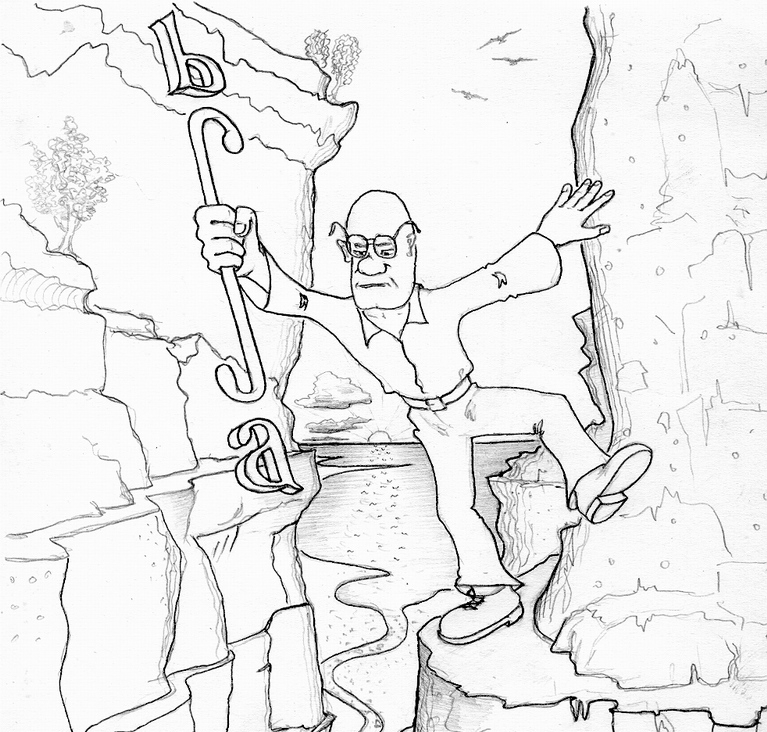
\includegraphics[width=0.35\textwidth]{pict.png}
\it
\caption{Взятие интеграла над пропастью во время захода Солнца} \label{f1}
\end{figure}
Здесь идет текст третьей главы. Здесь идет текст третьей главы. Здесь идет текст третьей главы.
Здесь идет текст третьей главы. Здесь идет текст третьей главы. Здесь идет текст третьей главы.
Здесь идет текст третьей главы. Здесь идет текст третьей главы. Здесь идет текст третьей главы.
Сслыка на литературу \cite{Conference}

\header{Часть 3}

Здесь идет текст третьей главы. Здесь идет текст третьей главы. Здесь идет текст третьей главы.
Здесь идет текст третьей главы. Здесь идет текст третьей главы. Здесь идет текст третьей главы.
Здесь идет текст третьей главы. Здесь идет текст третьей главы. Здесь идет текст третьей главы.
Здесь идет текст третьей главы. Здесь идет текст третьей главы. Здесь идет текст третьей главы.
Здесь идет текст третьей главы. Здесь идет текст третьей главы. Здесь идет текст третьей главы.
Здесь идет текст третьей главы. Здесь идет текст третьей главы. Здесь идет текст третьей главы.
Сслыка на литературу \cite{Article}

\header{Заключение}

В работе рассмотрен случай статистического оценивания неизвестного параметра сдвига, основанный на выборочной медиане, построенной по выборкам случайного объема. С помощью понятия дефекта проведено асимптотическое сравнение качества такой оценки. Получены явные формулы для асимптотического дефекта, имеющего смысл необходимого добавочного числа наблюдений. Подробно рассмотрен случай, когда случайный объем выборки имеет биномиальное, пуассоновское и трехточечное симметричное распределения~\cite{webSite}.


\bigskip\bigskip\def\refname{\centerline{Список литературы}}


\bibliographystyle{ugost2008.bst}  %% стилевой файл для оформления по ГОСТу
\bibliography{cites}


\bigskip\medskip{\centerline{\bf Библиографическая ссылка}}\medskip
{Бенинг В.Е., Савушкин В.А. О дефекте выборочной медианы в случае выборок случайного объема // Вестник ТвГУ. Серия: Прикладная математика. 2016. №~2. С.~\pages.}

\bigskip\medskip{\centerline{\bf Сведения об авторах}}
\begin{enumerate}[1.]
\item {\bf Бенинг Владимир Евгеньевич}\\
профессор кафедры математической статистики факультета вычислительной математики и кибернетики Московского 
государственного университета им. М.В. Ломоносова, старший научный сотрудник ИПИ РАН.

\vspace{1mm}
{\it Россия, 119992, г. Москва, ГСП-1, Воробьевы горы, МГУ им. М.В. Ломоносова. E-mail: ivanov@yandex.ru.} 
\item {\bf Савушкин Владислав Андреевич}\\
ассистент кафедры прикладной математики и информатики факультета естественных  и инженерных наук государственного университета Природы, Общества и Человека <<Дубна>>.

\vspace{1mm}
{\it Россия, 141982, Московская область, г. Дубна, улица Университетская, д. 19, Университет Дубна. E-mail: sidorov@mail.ru.} 
\end{enumerate} 

\end{document}